\documentclass[11pt]{article}
\usepackage{lmodern}
\usepackage[T1]{fontenc}
\usepackage[utf8]{inputenc}
\usepackage[a4paper,margin=2.4cm]{geometry}
\usepackage{graphicx}
\usepackage{float}
\usepackage[hidelinks]{hyperref}
\usepackage[round]{natbib}
\setlength{\parskip}{0.5ex}
\graphicspath{{figures/}}

\begin{document}

% ===================== COVER (not counted) =====================
\begin{titlepage}
\centering
\vspace*{3cm}
{\LARGE\bfseries Renewables in the UK:\\[2mm] Capacity, Geography and the Role of Policy\par}
\vspace{1.5cm}
{\large DSM050 Data Visualisation --- Midterm Coursework\par}
\vspace{0.5cm}
{\large MSc Data Science\par}
\vspace{2cm}
{\large [William Sidney-Roberts / ws160@london.ac.uk]\par}
\vspace{2cm}
{\normalsize Word count (main body): \textasciitilde2{,}250\par}
{\normalsize Code and data: \url{https://github.com/peaceman-per/DV-CW1-Reattempt-2026-S4}\par}
\vfill
\end{titlepage}

% ===================== 1. RESEARCH CONTEXT =====================
\section{Research context and problem definition}

The decarbonisation of electricity is central to the United Kingdom's climate strategy. In 2008 the UK parliament enacted the Climate Change Act with the aim to cut emissions by 80\% from a 1990s baseline by the year 2050. This act was then amended --- following advice from the climate change committee formed from the original 2008 act \citep{ccc2019} --- to the elimination of \textbf{all} carbon emissions by 2050. The subsequent Net Zero Strategy placed the rapid expansion of renewables --- and offshore wind in particular --- as the heart of delivery \citep{netzero2021}. Understanding \emph{how} the UK's renewable assets have actually grown, where it sits, and what policy levers designed it is therefore of direct interest to the audience for this report: energy-policy analysts and industry stakeholders who need an evidence-based picture of the transition, rather than headline slogans.

A few domain concepts frame the analysis. \textbf{Installed capacity} (measured in megawatts, MW) is the maximum power a project is designed to deliver; it is distinct from \emph{generation} (energy produced over time, MWh), which this dataset does not record --- an important limitation returned to below. Projects progress through various levels of \textbf{development status} (here grouped as operational, pending or terminated). Government support has run through three successive schemes: the \textbf{Renewables Obligation} (RO, 2002), \textbf{Feed-in Tariffs} (FiT, 2010, aimed at small-scale generation) and \textbf{Contracts for Difference} (CfD, 2014, allocated through competitive auction rounds AR1--AR7). Geography is reported at the \textbf{NUTS1} region level where England is split into 9 regions and 3 others represent the other countries in the UK (e.g. Scotland, Norther Ireland, South East, East Midlands, etc.).

The objective is to build a clear, honest and reproducible visual account of the current and past UK renewable energy landscape that lets this audience explore three things: the changing technology mix, its regional distribution over time, and the real impact of policy. The analysis deliberately foregrounds design choices and limitations, so that what the charts show --- and what they cannot show --- is transparent and therefore honest.

% ===================== 2. RESEARCH QUESTIONS =====================
\section{Research questions}

The investigation is aimed at three questions, chosen to be answerable with the available data and to build from description toward explanation:

\begin{itemize}
  \item \textbf{RQ1 --- Technology mix and growth.} How has the composition of the UK's renewable energy \emph{capacity} evolved over time, and to what extent has wind (offshore versus onshore) driven that change relative to solar and other sources?
  \item \textbf{RQ2 --- Regional distribution.} How is renewable capacity distributed across UK regions, and how has that geography evolved?
  \item \textbf{RQ3 --- Government support.} How are the support schemes (CfD, RO, FiT) associated with the scale and technology mix of renewable projects?
\end{itemize}

These questions matter because they depend on one-another. The technology mix is a policy artefact: the FiT drove a rapid, small-scale solar boom \citep{cherrington2013}, while the CfD auctions were designed to bring forward nation-scale offshore wind and were successful in driving strike prices down \citep{welisch2020}. Geography is not neutral either --- onshore wind is heavily concentrated in Scotland, with consequences for grid balancing and spatial ``smoothing'' of distribution \citep{commin2017}, while offshore wind has its own distinct spatial and temporal signature \citep{potisomporn2022}. Analysing each question in the same report allows us to see the bigger picture each question is framed within.

% ===================== 3. DATA & PREPROCESSING =====================
\section{Dataset and preprocessing}

The analysis uses the Renewable Energy Planning Database (REPD), A record of all renewable energy projects in the UK with a capacity above 150\,kW maintained by the Department for Energy Security and Net Zero \citep{repd2026}. The database as of Q1 2026 contains 14,316 projects across 53 fields covering technology, capacity, location, dates and support scheme.

Preprocessing (in \texttt{pandas}) proceeded in stages, each aimed at making the data safe, quick and easy to aggregate. First, roughly thirty planning- and legal-status columns irrelevant to \emph{what has been built} were dropped, and \texttt{Ref ID} moved to the index. Second, the many raw development-status values were distilled into three analytically meaningful groups (operational, pending, terminated), and the technology field was consolidated (for example, co-firing and dedicated biomass into ``Biomass''; large and small hydro into ``Hydro''), with pure storage technologies removed so that only generation remains. Third, numeric fields were coerced to numbers with non-applicable blanks set to zero, and text location fields were standardised.

Missing values were handled by meaning, not mechanically. The \texttt{Operational} date is legitimately blank for projects that never became operational, so those blanks were preserved; only the small residual of rows missing genuine identifying information were dropped. Because most numeric fields are scheme-specific and therefore sparse (mostly zero), classical dimensionality reduction such as PCA is a poor fit; instead, dimensionality is managed by \emph{feature selection}, answering each question with the few variables that carry relevant signal (capacity, technology, region, date, scheme).

Refreshing last year's workflow onto the newer data surfaced three instances of data drift that would otherwise have secretly corrupted the previous analysis: a new development-status value (\texttt{Application Granted}); two new CfD auction rounds (AR7, AR7a); and an inconsistent capitalisation (\texttt{Investment Contract}). Detecting and mapping these recovered roughly 190 projects that a naive re-run would have dropped --- a reminder that reproducibility across new data requires validation, not blind reuse.

% ===================== 4. EDA & VISUALISATION =====================
\section{Exploratory data analysis and visualisation}

The key variables span three measurement types: \emph{nominal} (technology type, country, region), \emph{ordinal} (CfD allocation round)\footnote{Allocation rounds are treated as ordinal rather than nominal because they are administered sequentially over time (AR1 through AR7a), so round number is a monotonic proxy for when a project entered the scheme, not just an unordered label.} and \emph{numerical} (installed capacity and related continuous fields). Figure~\ref{fig:eda} summarises the categorical variables. By project \emph{count}, solar dominates, followed by onshore wind; England hosts most projects; and the large majority of projects sit outside the CfD scheme, with past CfD rounds generally accepting fewer projects than future rounds. The numeric fields are highly sparse, which motivated the feature-selection approach above.

Visualisation choices follow established guidance: consistent, meaningful colour; explanatory titles; and scales chosen to reveal rather than distort \citep{kelleher2011,qin2020}. A single technology colour map is reused across every figure so the reader learns it once. Capacity, which is highly skewed, is shown on log axes where distributions are compared, and a shared colour scale is used across the regional snapshots so that growth is visible rather than re-normalised away.

\begin{figure}[H]
  \centering
  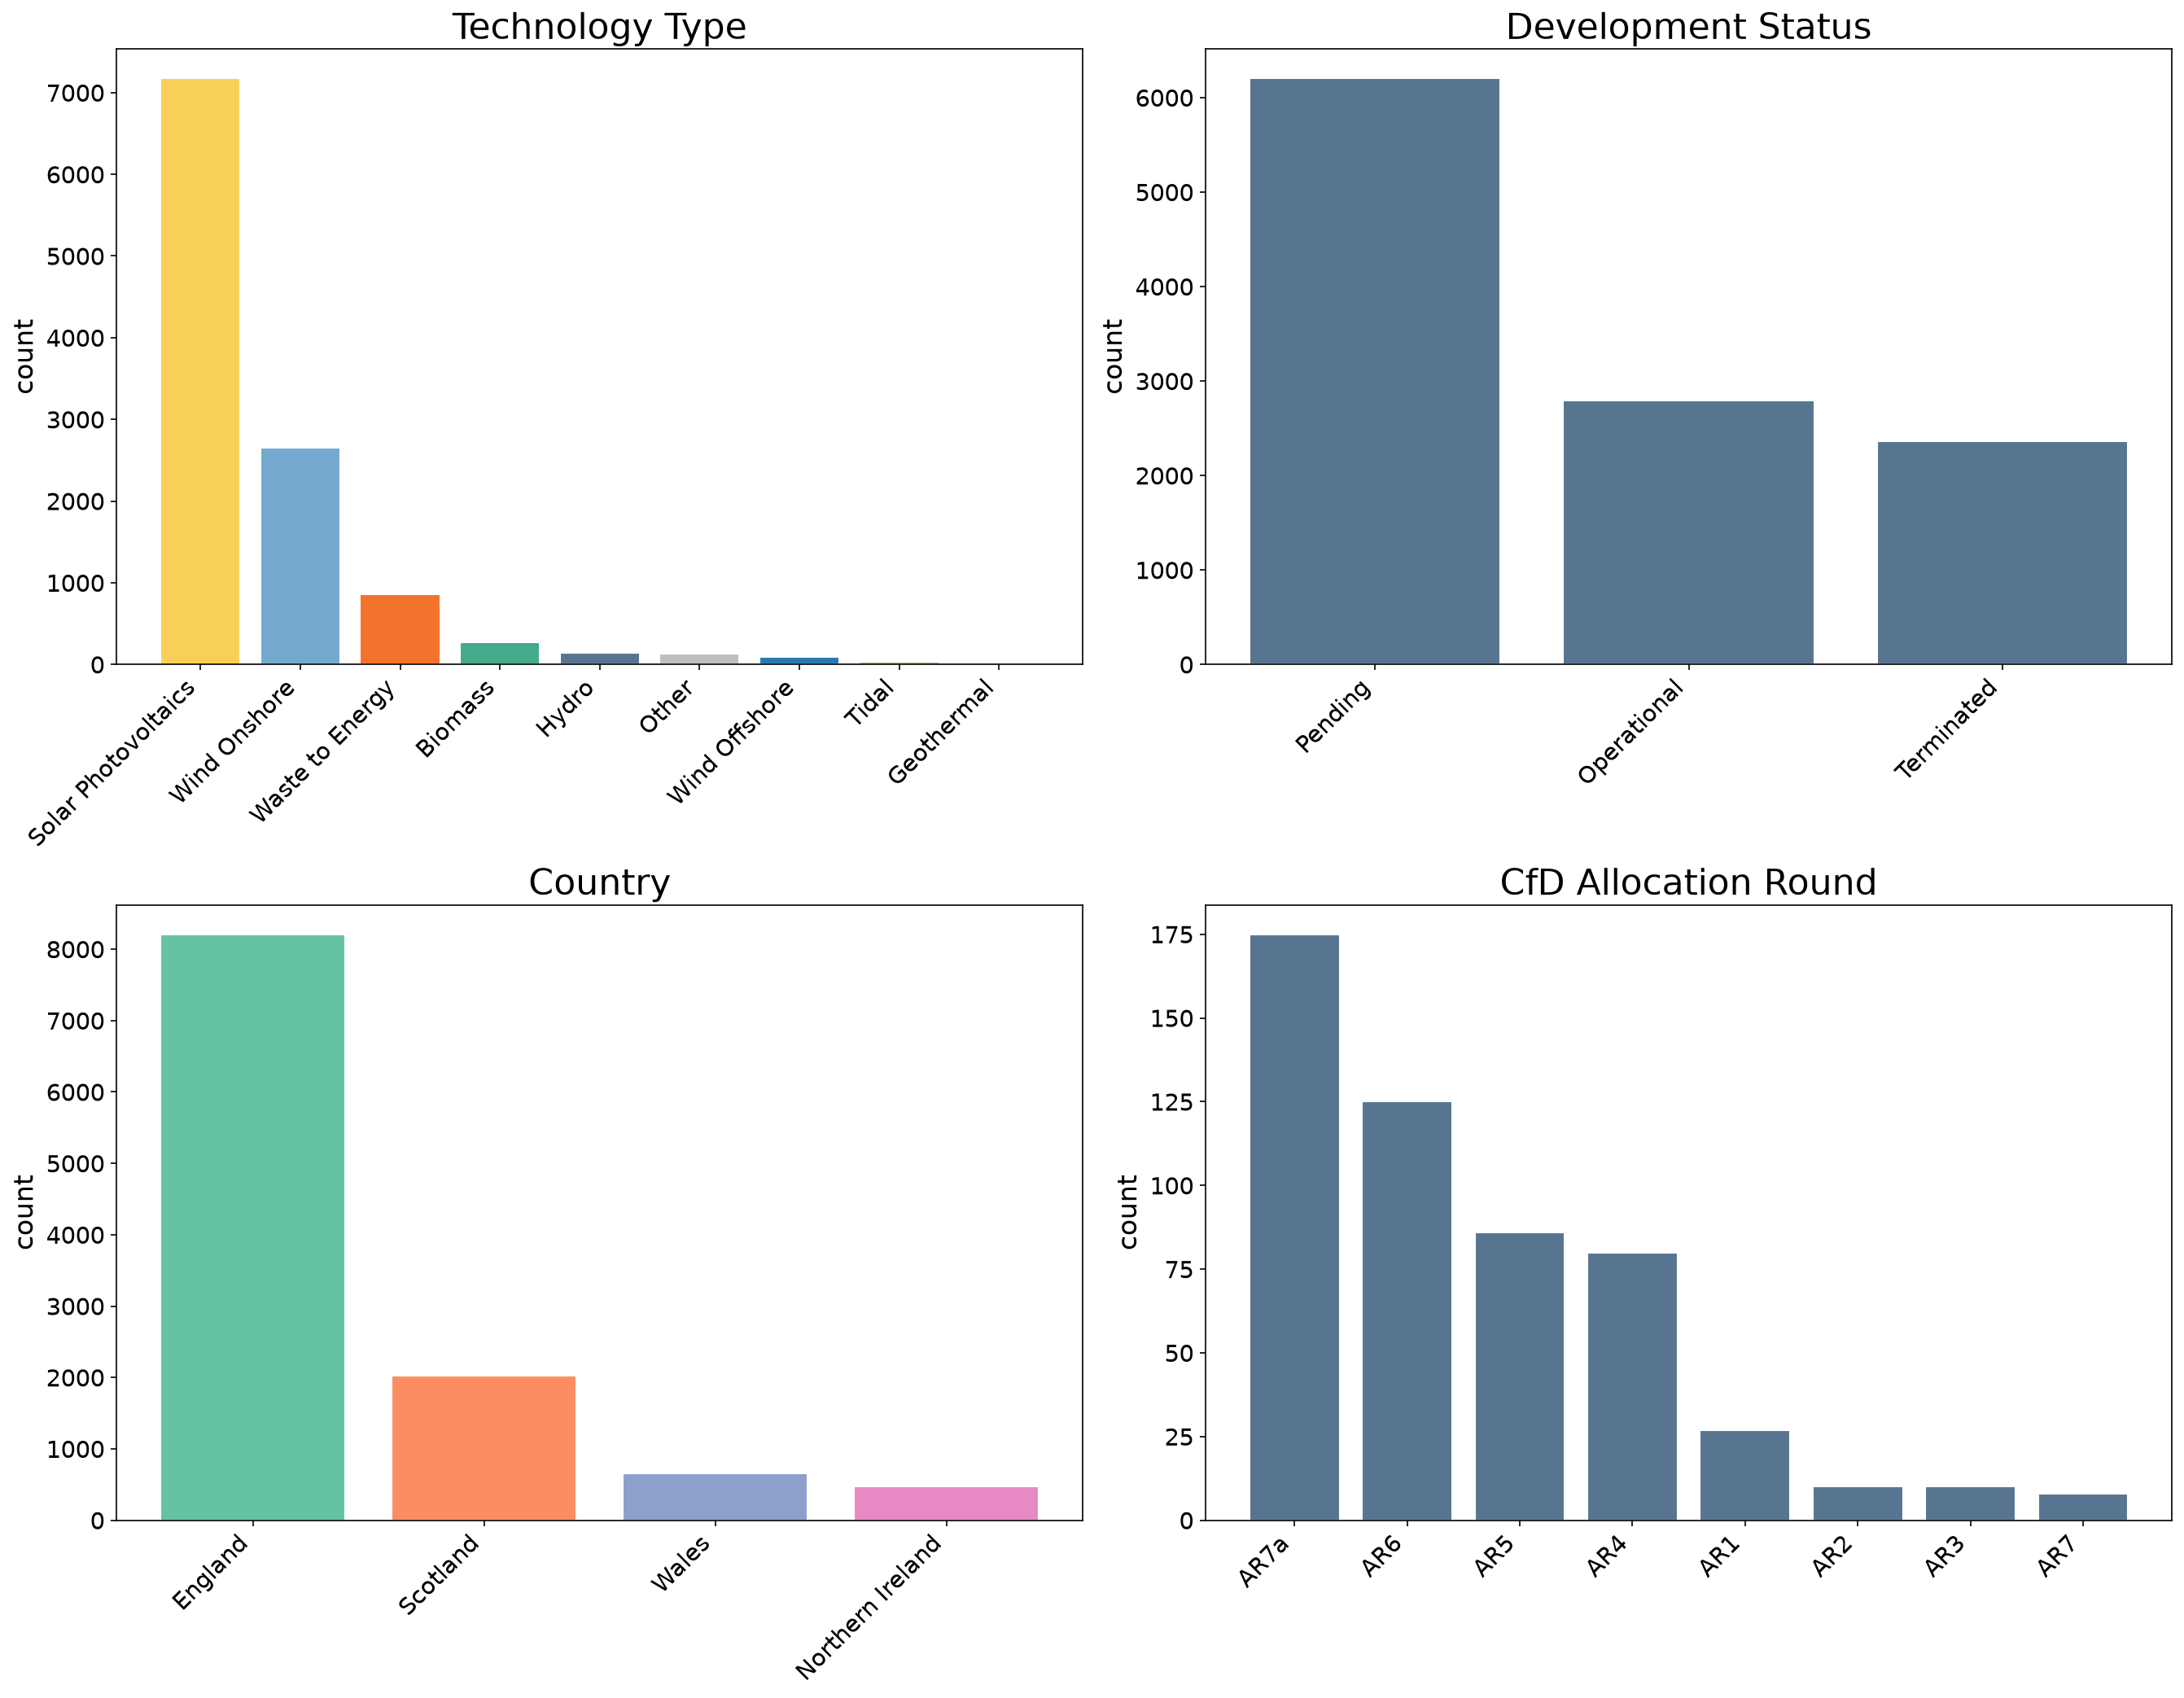
\includegraphics[width=0.92\linewidth]{eda_categorical_counts.png}
  \caption{Distribution of the key categorical variables. Counts are dominated by small solar projects, but counts and \emph{capacity} tell very different stories (see Figure~\ref{fig:rq1}). The CfD allocation-round panel omits the \texttt{None} category ($n=10{,}840$ projects, 95.4\%) so the funded rounds are legible --- that most projects sit outside CfD is itself the point.}
  \label{fig:eda}
\end{figure}


For RQ1, a pie chart gives the current capacity share and paired stacked-area charts trace the mix over time by both project count and capacity (Figure~\ref{fig:rq1}). For RQ2, because offshore wind is not attributable to a land region, the design maps the twelve land regions as time-stratified choropleths while reporting offshore separately on the same colour scale (Figure~\ref{fig:rq2}); an interactive time-slider version accompanies the notebook. For RQ3, a strip-and-box plot relates capacity to CfD round, coloured by technology (Figure~\ref{fig:rq3_round}); a normalised stacked bar then shows the technology mix within each round, and a heatmap compares median project size under each scheme against a time-matched non-scheme baseline (Figure~\ref{fig:rq3}).

\begin{figure}[H]
  \centering
  \begin{minipage}{0.54\linewidth}\centering
    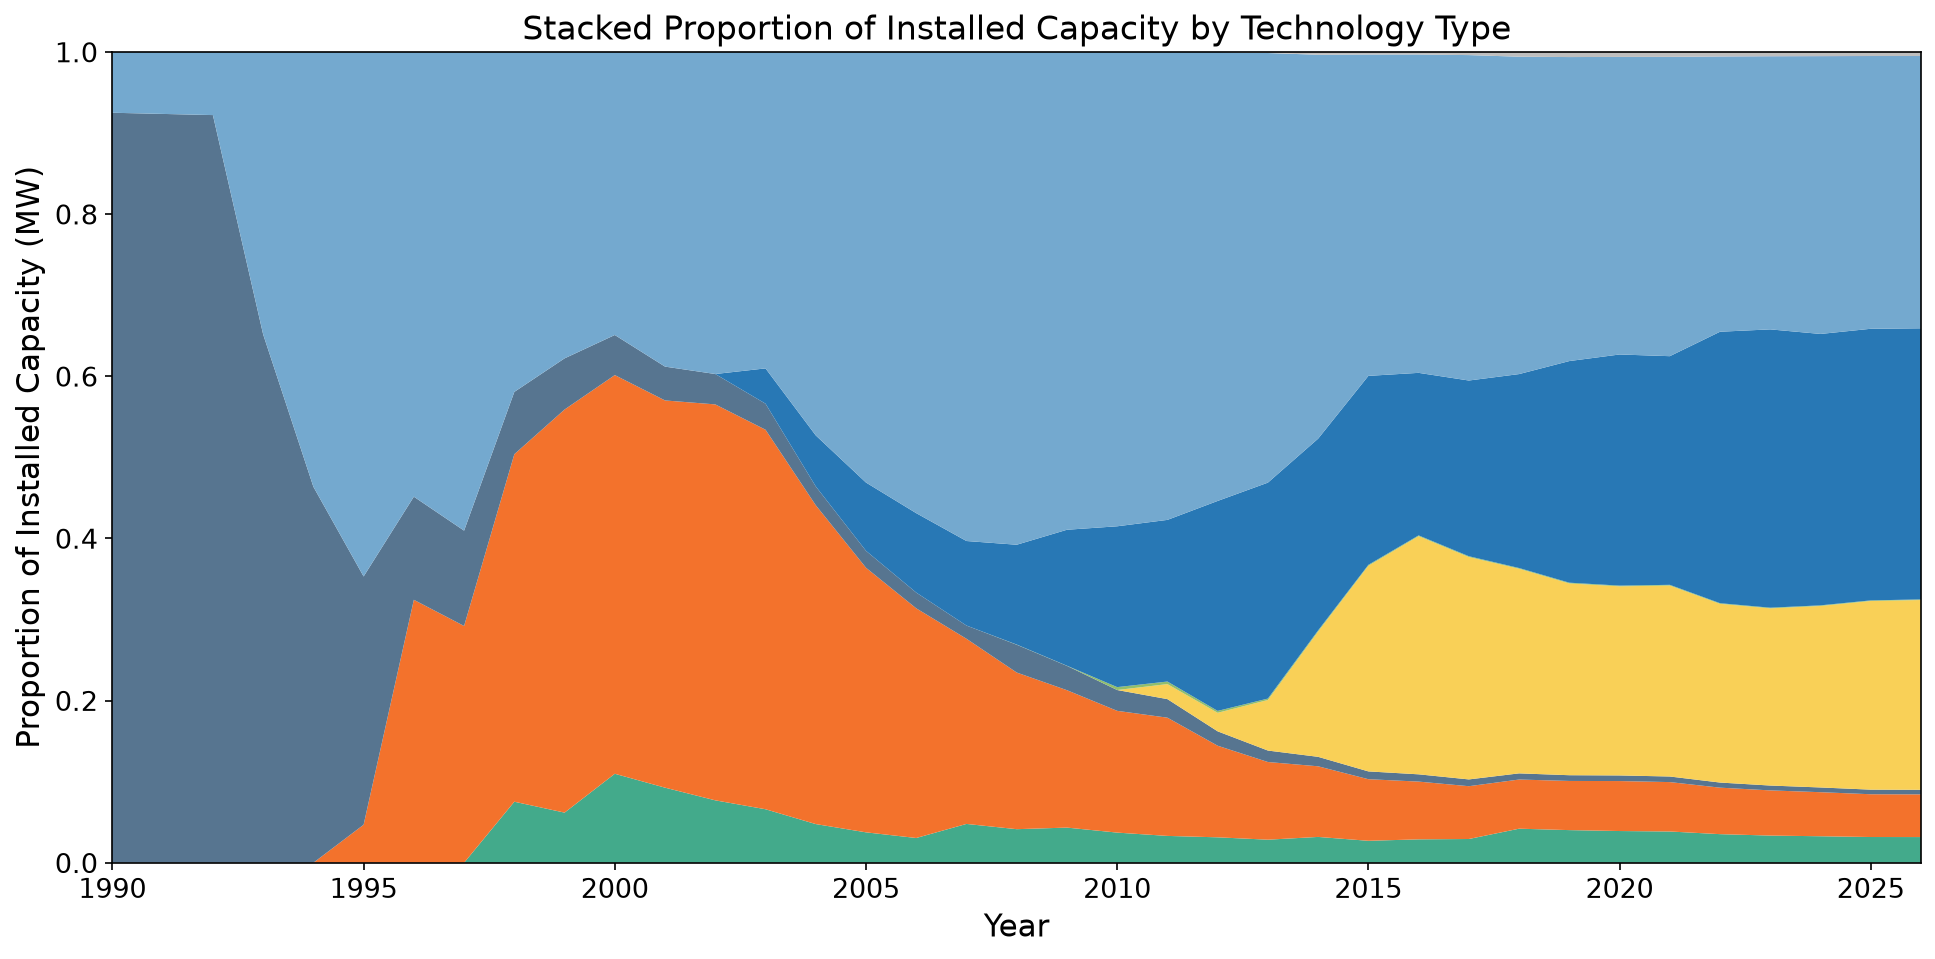
\includegraphics[width=\linewidth]{rq1_capacity_stacked_area.png}
  \end{minipage}\hfill
  \begin{minipage}{0.44\linewidth}\centering
    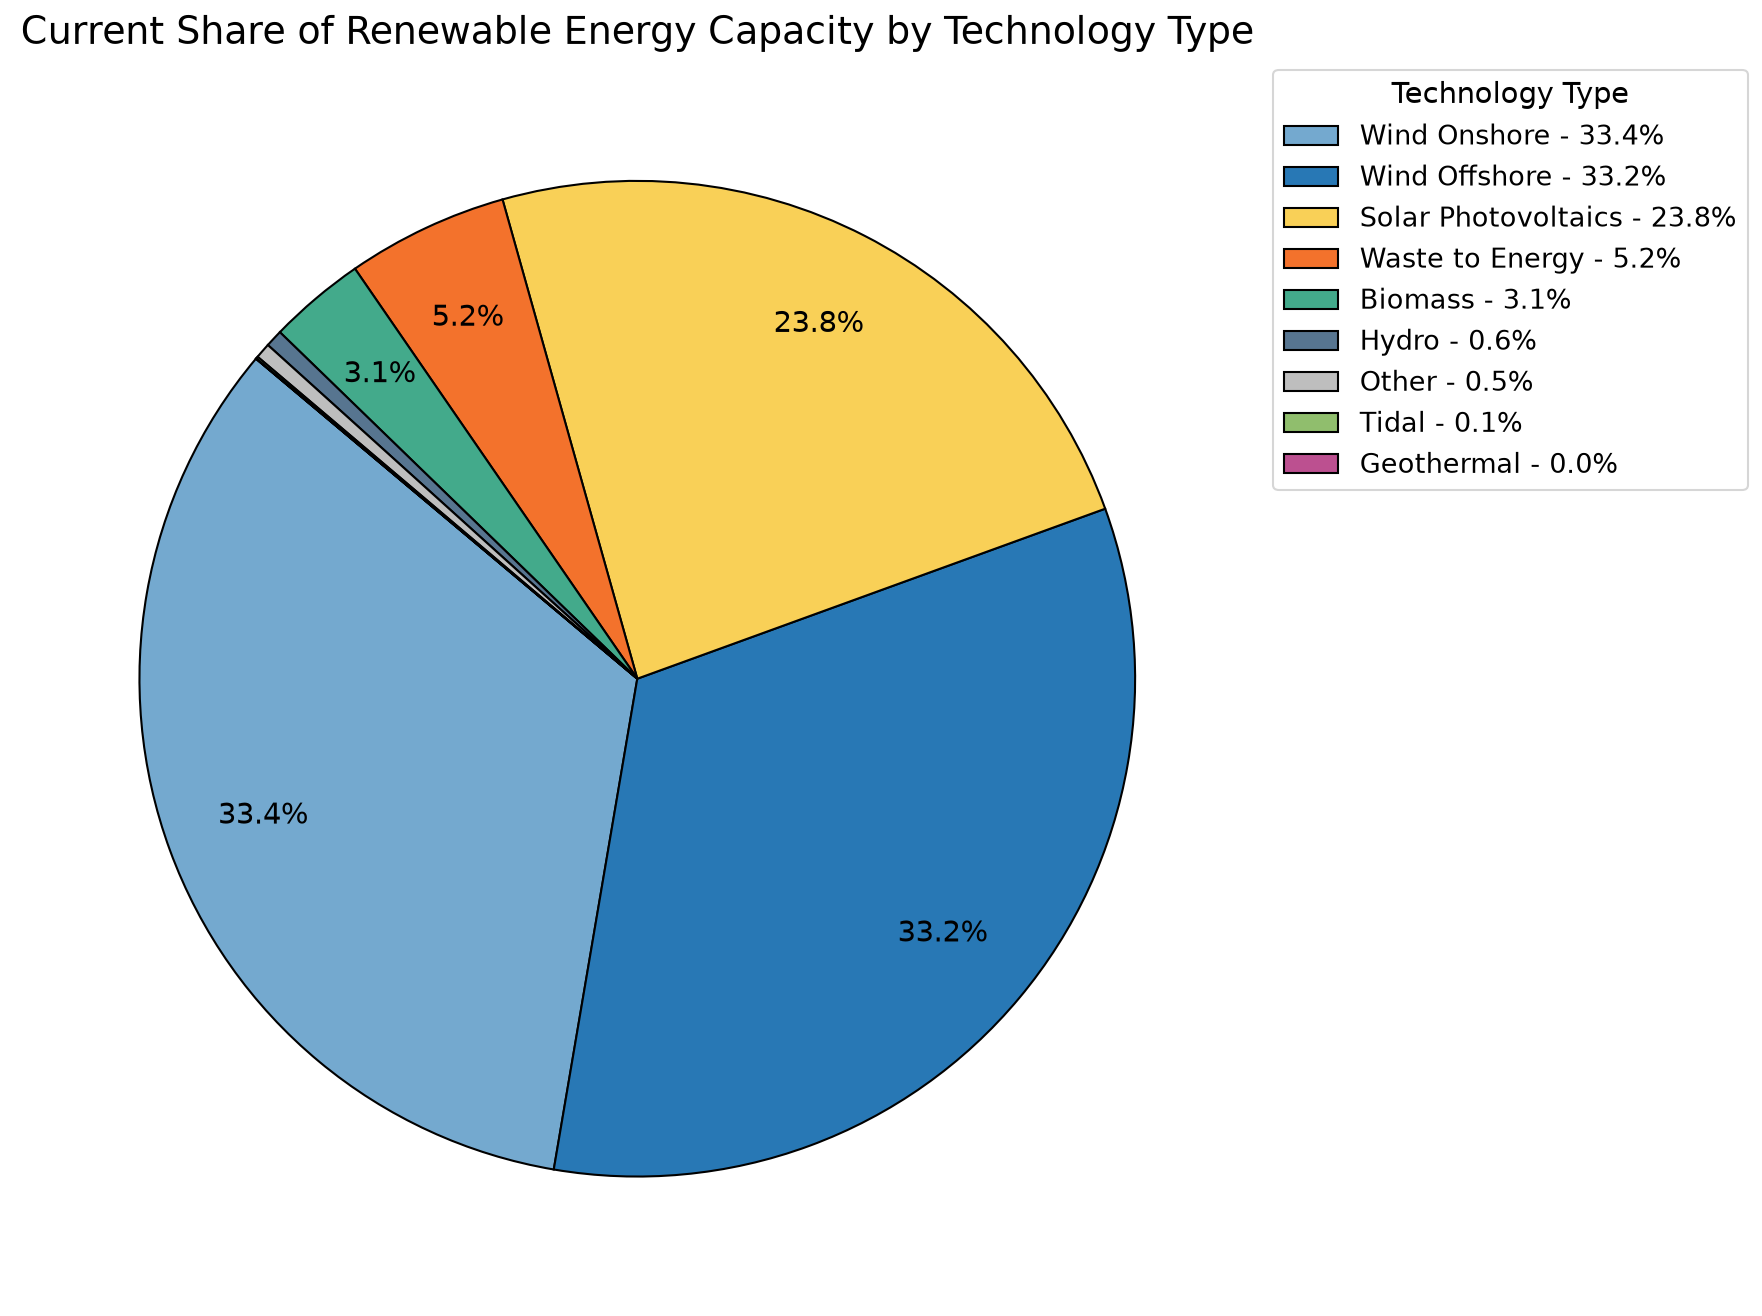
\includegraphics[width=\linewidth]{rq1_capacity_share_pie.png}
  \end{minipage}
  \caption{RQ1. Left: the evolving capacity mix, 1990--2026. Right: current share of operational capacity by technology. Wind holds roughly two-thirds of capacity; the visible waves track successive policy regimes. Both panels use the same technology colour map, so a single legend (on the pie) serves both.}
  \label{fig:rq1}
\end{figure}

\begin{figure}[H]
  \centering
  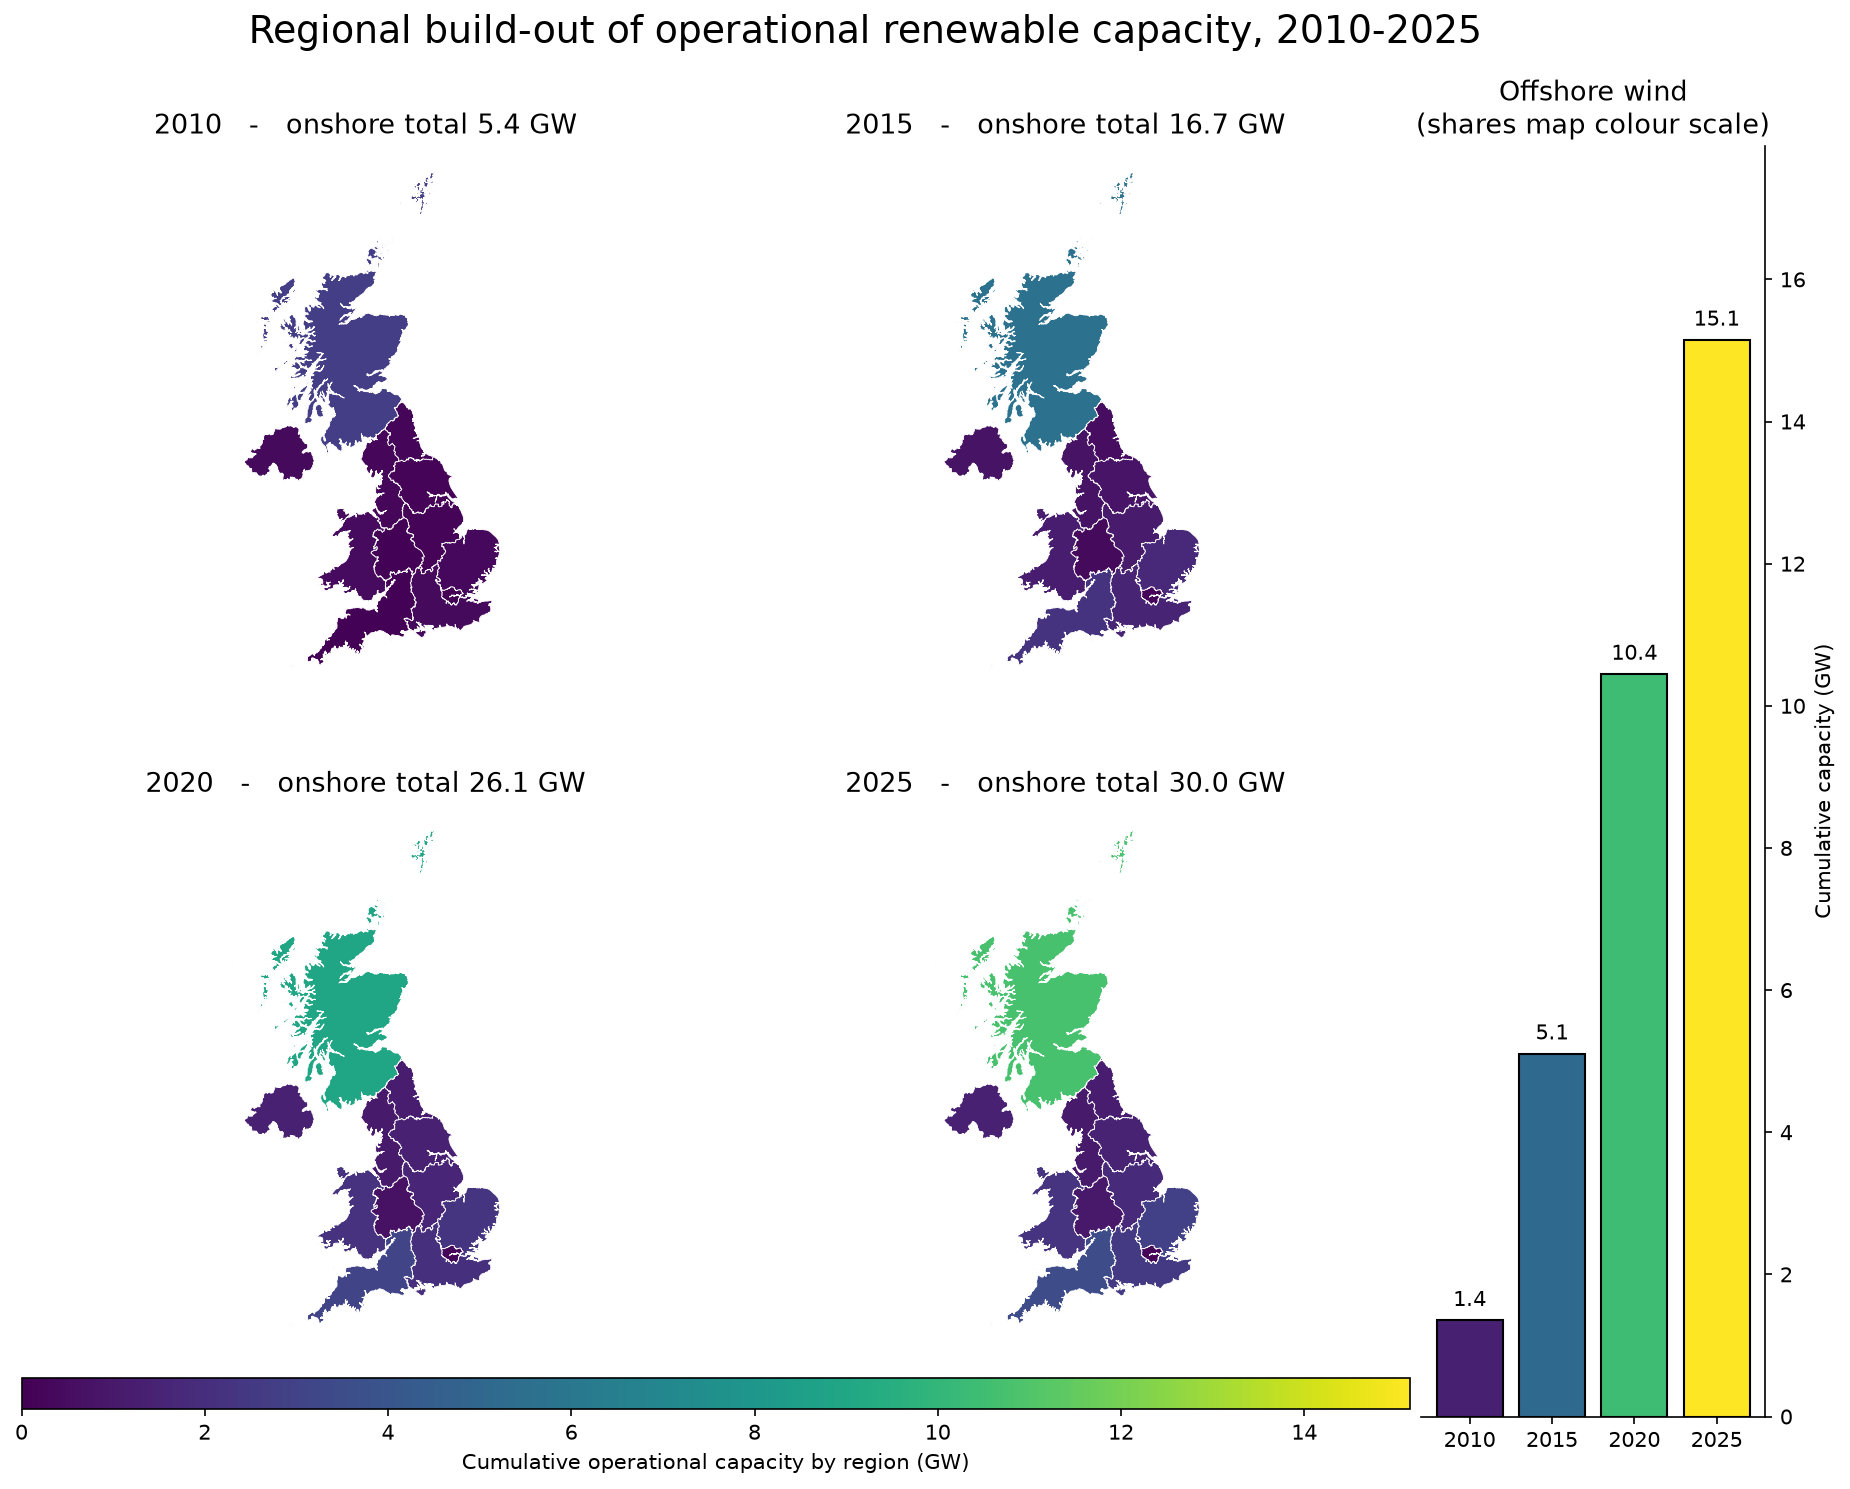
\includegraphics[width=0.95\linewidth]{rq2_regional_snapshots_2x2.png}
  \caption{RQ2. Cumulative operational capacity by region at four snapshots, with offshore wind (not a land region) shown on the same colour scale. Scotland leads onshore; offshore overtakes every land region by 2025.}
  \label{fig:rq2}
\end{figure}

\begin{figure}[H]
  \centering
  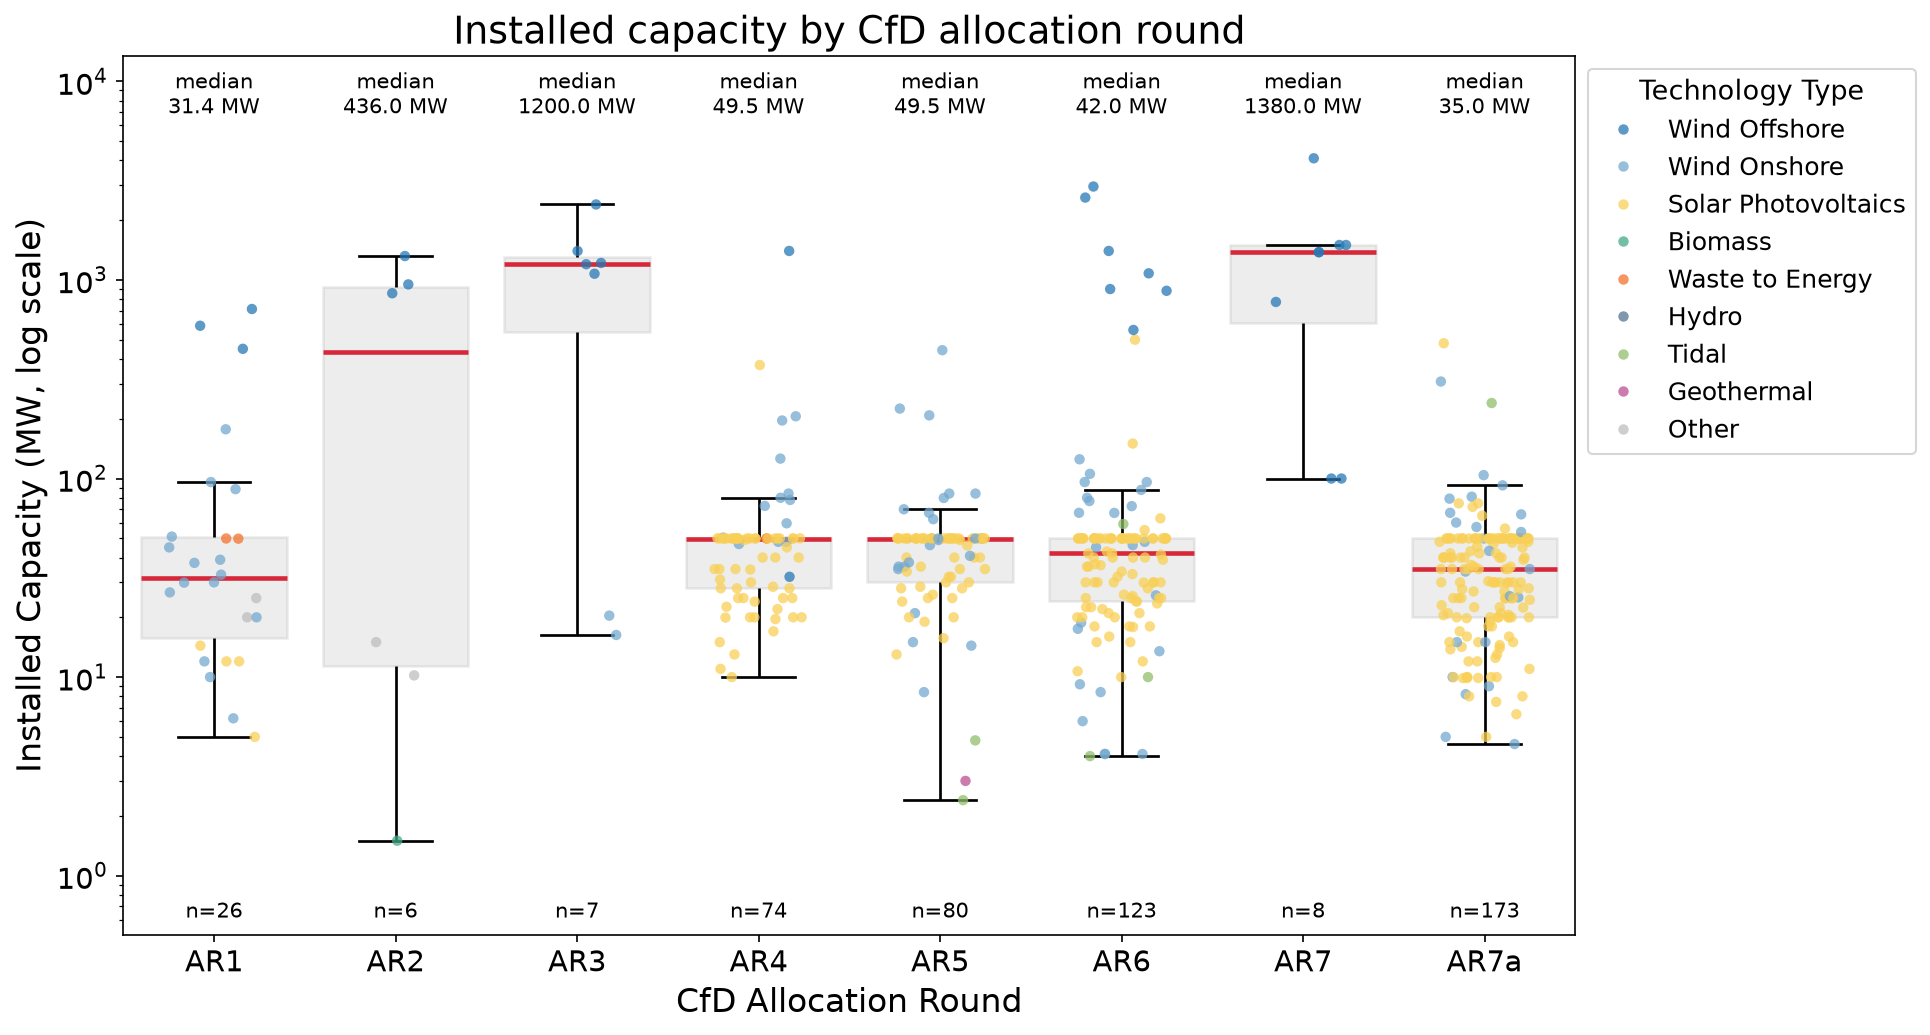
\includegraphics[width=0.92\linewidth]{rq3_capacity_by_cfd_round.png}
  \caption{Installed capacity by CfD allocation round (chronological; the \texttt{None} category, 95.4\% of projects, is omitted for the same reason as in Figure~\ref{fig:eda}). Each point is a project, coloured by technology; the overlaid box marks the median and interquartile range. Median and sample size are annotated per round.}
  \label{fig:rq3_round}
\end{figure}

\begin{figure}[H]
  \centering
  \begin{minipage}{0.58\linewidth}\centering
    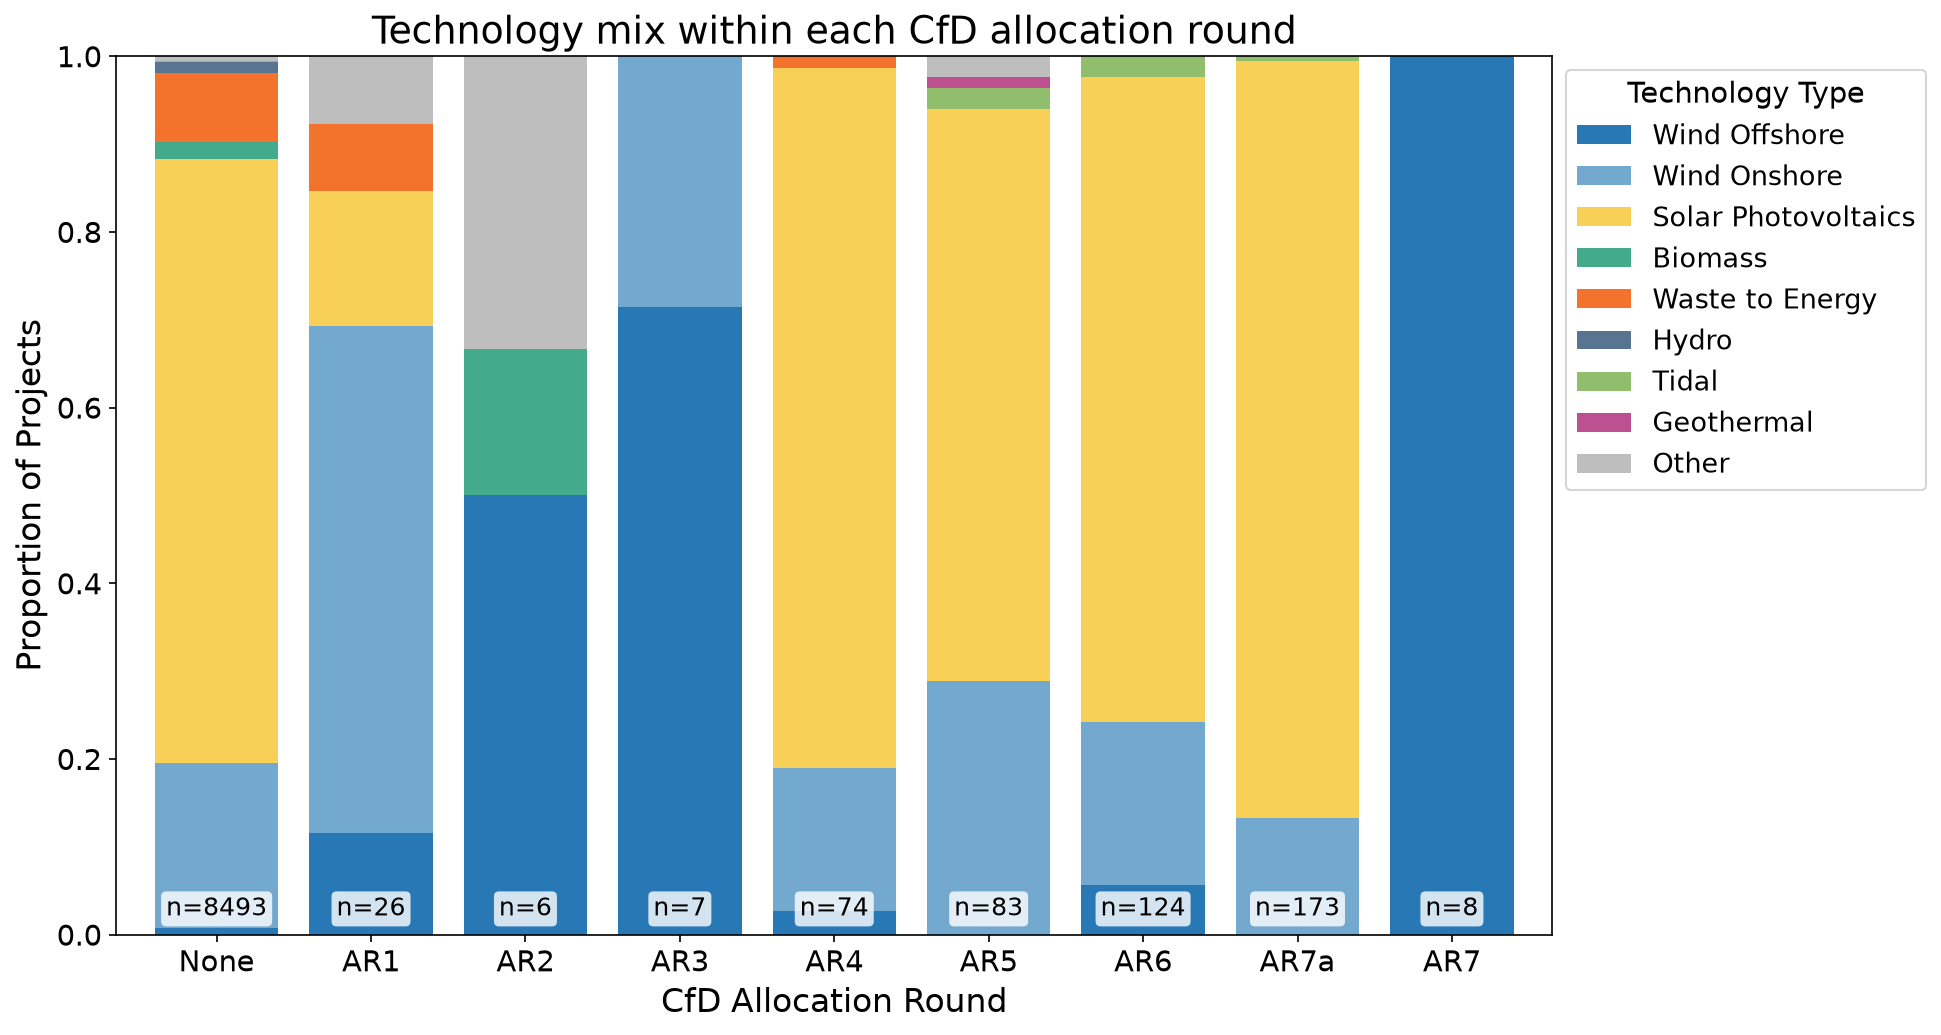
\includegraphics[width=\linewidth]{rq3_cfd_round_vs_tech.png}
  \end{minipage}\hfill
  \begin{minipage}{0.40\linewidth}\centering
    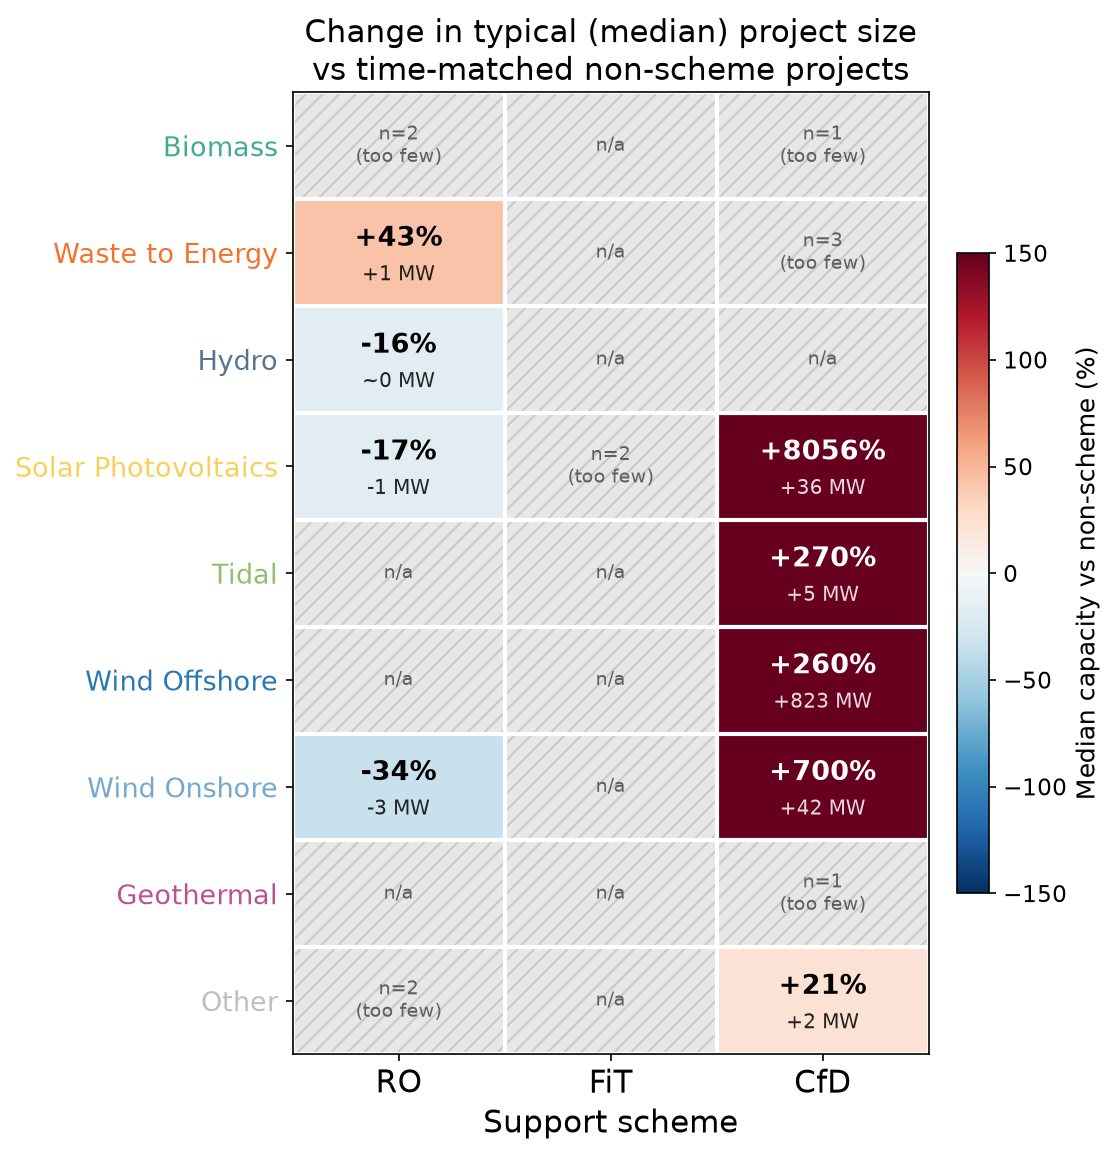
\includegraphics[width=\linewidth]{rq3_capacity_by_scheme.png}
  \end{minipage}
  \caption{RQ3. Left: technology mix within each CfD round (project counts annotated); the newest round, AR7, is entirely offshore wind. Right: heatmap of the scheme-associated change in typical (median) project size by technology, each scheme time-matched to non-scheme projects active in its own eligibility window (diverging scale, centred at zero). Cells with fewer than five in-scheme projects, or none, are hatched. Under CfD, projects are far larger than their contemporaries across technologies; under RO the premium is small or negative once like-for-like periods are compared.}
  \label{fig:rq3}
\end{figure}


% ===================== 5. INTERPRETATION =====================
\section{Interpretation and discussion}

\textbf{RQ1: capacity is not project count.} The most important insight from Figure~\ref{fig:eda} and Figure~\ref{fig:rq1} is the gap between the two framings. Solar accounts for the most \emph{projects}, yet wind (onshore and offshore) supplies about two-thirds of operational \emph{capacity}, because individual wind farms are far larger than the numerous small solar sites. The stacked-area chart in Figure~\ref{fig:rq1} reads as a history of policy: an early Onshore boom shortly followed in 95/96 by a waste to energy peak, the mid-2000s re-rise of onshore wind under the RO and start of offshore elevation, the early-2010s solar spark that followed the FiT\citep{cherrington2013} then surging in ~2015, and the steady climb to strength of offshore wind during 05-25. For a policy audience the implication is concrete: capacity targets are being met by a driving force of a minority of very large wind assets, so the fleet's fortunes are increasingly tied to the economics of that one technology \citep{potisomporn2022}.

\textbf{RQ2: the map hides the main story.}\label{sec:rq2} Figure~\ref{fig:rq2} shows Scotland dominating land-based capacity throughout, with the south of England filling in later. This concentration is not costless: heavy clustering of capacity in one part of the country reduces the spatial ``smoothing'' of output and raises grid-balancing challenges \citep{commin2017}. But the decisive point is what a regional map \emph{cannot} show. Offshore wind --- roughly a third of all operational capacity --- sits in no NUTS1 region, and it is the single largest and fastest-growing source (1.4\,GW in 2010 to 15.1\,GW in 2025). Presenting it in a side panel rather than dropping it (as a naive regional analysis might) keeps the national growth engine visible. The audience takeaway is that any regional framing of the transition is incomplete unless offshore is treated explicitly.

This is not a hypothetical concern. Individually attributing the four largest operational or under-construction offshore projects to their actual grid connection points --- East Anglia ONE and the planned East Anglia Two/Three at Bramford, Suffolk \citep{eastanglia_bramford}; Hornsea One and Two at North Killingholme \citep{hornsea_killingholme}; Hornsea Three at Norwich Main \citep{hornsea3_norwich}; and the Walney Extension at Heysham \citep{walney_heysham} --- would shift several gigawatts onto East of England, Yorkshire and The Humber, and North West England: precisely the regions the current land-only map makes look comparatively unremarkable. This is a reminder that Figure~\ref{fig:rq2}'s regional framing, however carefully caveated, still risks understating England's role in the offshore build-out to a reader who skims the map without reading the offshore panel alongside it.

\textbf{RQ3: policy selects for scale --- but the comparison matters.} Figure~\ref{fig:rq3} makes the role of support schemes clear. A naive comparison across the whole database suggests median project size climbs steeply from RO through FiT to CfD, but much of that gradient is an \emph{era} effect: RO-era projects are measured against a non-scheme pool later flooded with tiny sub-megawatt solar. The right-hand heatmap removes that confound by comparing each scheme only against \emph{contemporaneous} non-scheme projects of the same technology. Two things then stand out. First, the CfD premium is real and technology-wide: within their own eligibility window median CfD project are often multiple times larger than its non-scheme peers --- roughly $+700\%$ for onshore wind, $+260\%$ for offshore wind (an absolute gap of some 800\,MW), and larger still for utility-scale solar --- consistent with the scheme's design intent and its documented success in bringing down offshore-wind costs through competitive auctions \citep{welisch2020}. Second, RO shows little or even a \emph{negative} size premium once time-matched (about $-34\%$ for onshore wind, $-17\%$ for solar): RO did not select for scale in the way the flat comparison implied, and FiT cannot be judged at all here, as too few projects clear the database's size floor. The technology mix within rounds also shifts, and the newest round (AR7, 2025) is entirely offshore wind --- a clear signal of what policy desires. Set against this, the pending pipeline is enormous (122\,GW) yet a large share of historic projects are terminated; planning is a critical bottleneck, and the likelihood of refusal is shaped by project size, local demographics and proximity to existing turbines \citep{harper2019}. For policymakers, the message is that a large pipeline is not the same as delivered capacity.

\textbf{Limitations.} Several caveats bound these findings. The REPD records capacity, not generation, so ``share'' here means share of installed MW, not of electricity actually produced --- and this gap is not uniform across technologies: offshore wind's long-run load factor (around 43\%) is roughly 1.4$\times$ that of the UK wind fleet as a whole (31.3\%, DESNZ/DUKES) \citep{renewableuk_ukwed}, and both sit far above solar PV's, so a generation-weighted version of Figure~\ref{fig:rq1} would show wind and especially offshore wind capturing a materially larger share than its installed-MW share suggests, while solar's share would shrink; capacity alone cannot distinguish a technology that runs most of the time from one that runs only intermittently. Offshore capacity cannot be attributed to a land region --- not only because REPD does not record one, but because the choice of \emph{which} region would itself be arguable (nearest coastline? grid connection point? developer headquarters?); Section~\ref{sec:rq2} shows that under a connection-point attribution, several English regions currently reading as minor contributors would gain multiple gigawatts each, changing the map's shape substantially. Commissioning dates are missing for a minority of operational projects, slightly truncating the time series. The FiT scheme is under-represented because the database's 150\,kW floor excludes most domestic solar, leaving too few FiT projects to rate in the Figure~\ref{fig:rq3} heatmap; FiT is further confounded by its own 5\,MW eligibility cap, so a ``FiT versus no-scheme, same period'' contrast would partly reflect the economics of small projects in general rather than scheme choice alone. The pending pipeline figure reported alongside the dashboard is also naive in this sense: it is a simple sum of everything not yet operational, with no adjustment for the likelihood that a given project is actually delivered. Attrition is unlikely to be uniform --- offshore wind auctions in particular have seen entire rounds fail to attract bids or individual large projects cancelled outright \citep{carbonbrief_ar7} --- so a technology- or scheme-weighted pipeline estimate would likely be more informative, and probably smaller, than the headline number used here. Finally, the analysis is descriptive and associational, not causal: it identifies associations between policy and outcomes, not causal effects, and reflects a single Q1 2026 snapshot of a database that is revised over time.

% ===================== 6. DASHBOARD =====================
\section{Dashboard}

Figure~\ref{fig:dash} is a single-view dashboard designed for a policy or industry audience who need the headline picture at a glance. Its information hierarchy runs top-to-bottom: four key figures first (operational capacity, project count, wind share, and the pending pipeline), then the supporting detail --- the capacity mix, the growth trajectory, where capacity sits, and the policy lever. Colour is consistent with the rest of the report, offshore is highlighted where it matters, and each panel carries a plain-language title that states a finding rather than merely naming a variable. The aim is that a reader absorbs the transition's shape --- large, wind-dominated, offshore-led and policy-shaped --- in a few seconds, then drills into whichever panel is relevant to them.

\begin{figure}[H]
  \centering
  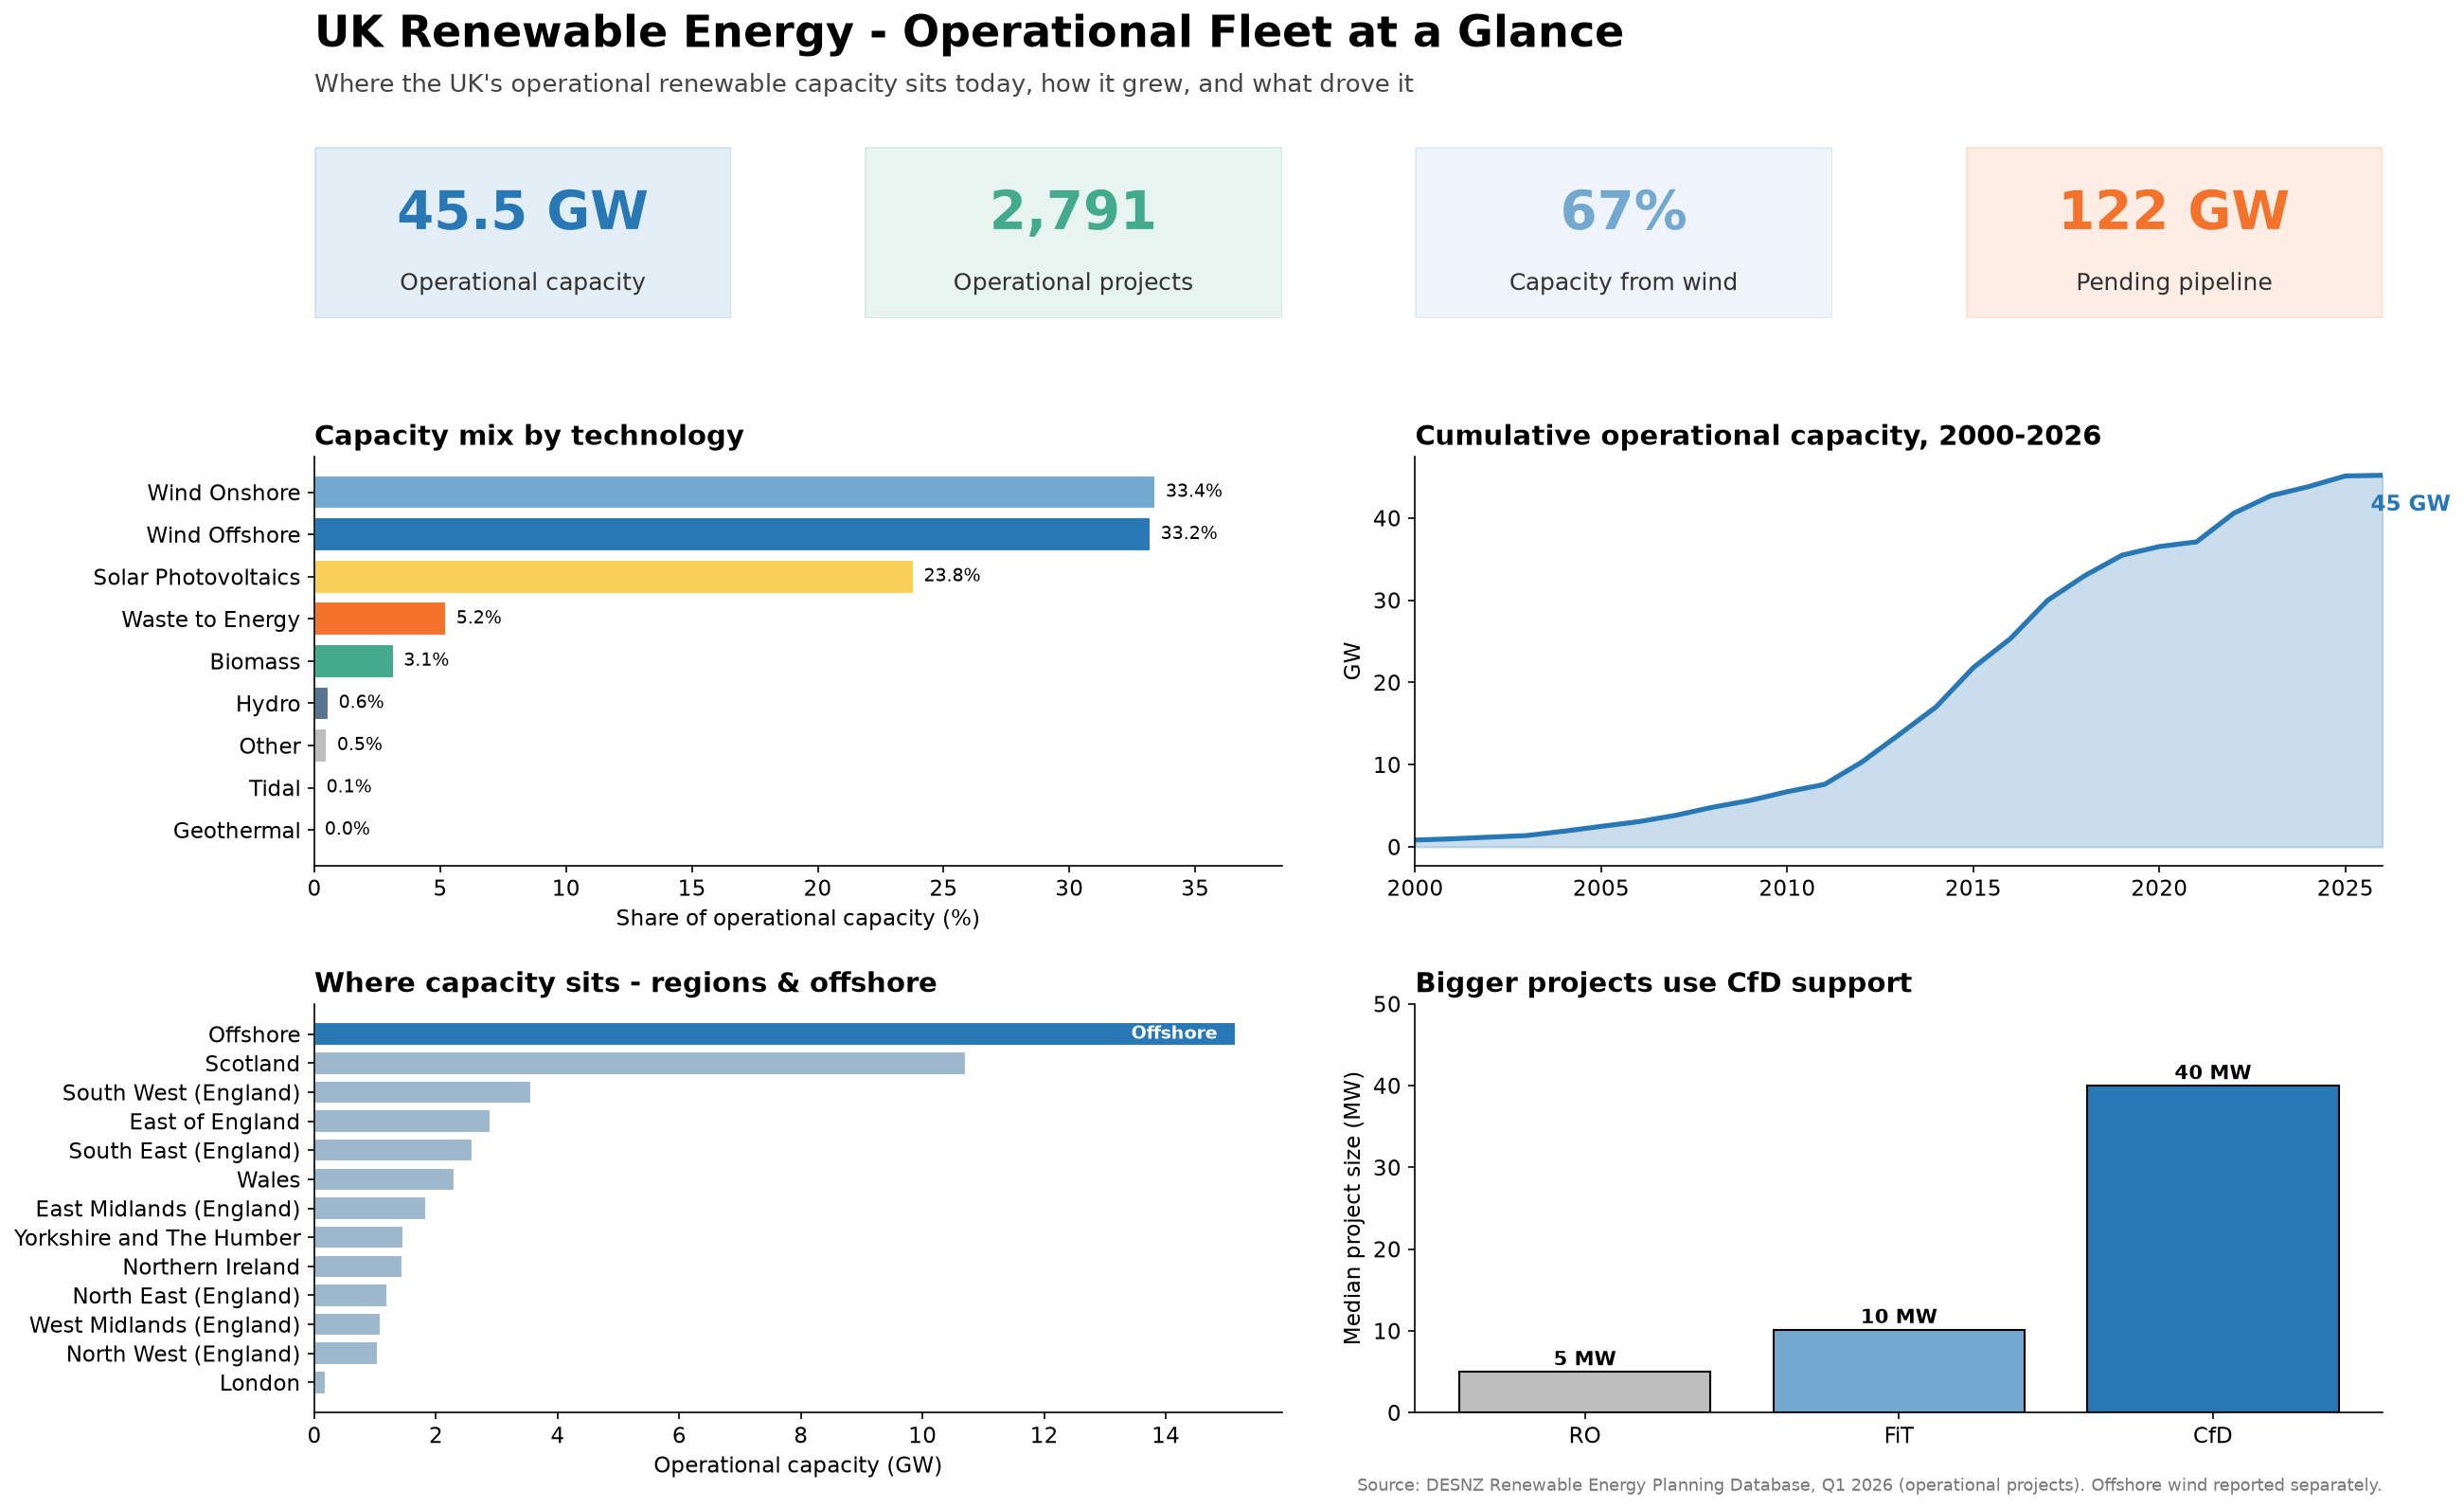
\includegraphics[width=0.98\linewidth]{dashboard.png}
  \caption{Summary dashboard of the UK's operational renewable fleet, designed for at-a-glance reading by a policy/industry audience.}
  \label{fig:dash}
\end{figure}

% ===================== REFERENCES (not counted) =====================
\bibliographystyle{plainnat}
\bibliography{references}

% ===================== APPENDIX (not counted) =====================
\appendix
\section{Declaration on the use of AI tools}

This coursework was produced with the assistance of AI tools (Anthropic Claude), AI assistance was used for:

\begin{itemize}
  \item \textbf{Socratic dialogue.} Talking through analytical and design choices --- e.g. how to handle offshore wind's lack of a land region, whether to use median or mean under skewed capacity distributions, and how to isolate a support scheme's effect from confounding era/technology trends --- with the AI posing questions and critiques rather than supplying answers directly.
  
  \item \textbf{Proofreading.} Identifying spelling, grammatical, and punctuation errors in the written report.
  
  \item \textbf{Prose critique.} Critiquing other writing elements, including structure, tone, and the correctness of research-related prose (e.g. whether a claim in the text was actually truly supported by the figure or source it referenced).
  
  \item \textbf{Code debugging and refactoring.} Debugging and suggesting refactorings of hand-written Python code in the accompanying Jupyter notebook, for readability and correctness rather than to generate new analysis from scratch.
\end{itemize}

All analytical decisions --- the research questions, the choice and interpretation of
visualisations, the handling of the data, and the conclusions drawn --- are my own. I have reviewed
and take responsibility for the entire submission. The original analysis on which this work builds
was my own prior coursework.

\end{document}
